\documentclass[review]{elsarticle}
\usepackage{comment}
\usepackage[utf8]{inputenc}
\usepackage[T1]{fontenc}
\usepackage{amsmath}
\usepackage{amsfonts}
\usepackage{amssymb}
\usepackage{multirow}
\usepackage{color}
\usepackage{graphicx}
\usepackage{booktabs}
\usepackage{longtable}
\usepackage{array}
\usepackage{tabularx}
\usepackage{rotating}
\usepackage{tikz}
\usetikzlibrary{shapes.geometric, arrows.meta, positioning, calc, fit, backgrounds}
\usepackage{pgfplots}
\pgfplotsset{compat=1.17}
\usepackage{mathtools}
\usepackage{verbatim}
\usepackage[
    colorlinks=true,
    citecolor=blue,
    linkcolor=blue,
    urlcolor=blue
]{hyperref}

\setlength{\parindent}{0pt}
\addtolength{\hoffset}{-0.50cm}
\addtolength{\textwidth}{2.0cm}
\addtolength{\voffset}{-0.50cm}

\newcommand{\dst}{\displaystyle}
\newtheorem{theorem}{Theorem}
\newtheorem{proposition}{Proposition}

\begin{document}

\begin{frontmatter}

\title{Scalable Coordination of Networked EV Charging Stations: \\
A Comprehensive Literature Review, Gap Analysis, and Novel Research Directions}

\author{Author Name}
\ead{author@university.edu}

\address{Department of Electrical Engineering, University Name, Country}

\begin{abstract}
The rapid proliferation of electric vehicles (EVs) poses unprecedented challenges for the coordinated operation of networked charging stations within power distribution networks. This report presents a comprehensive literature review covering over 100 references on the coordination of networked EV charging stations. We propose a structured taxonomy that classifies existing approaches into ten methodological families: distributed optimization (including ADMM-based methods), game-theoretic approaches, hierarchical coordination, reinforcement learning and deep learning, model predictive control, pricing and market dynamics, peer-to-peer transactive energy, vehicle-to-grid integration, aggregator-based management, and coupled transportation--power network optimization. Through a critical comparative analysis, we identify key research gaps, particularly the scalability limitations of ADMM-based distributed coordination when the number of stations grows large. To address these gaps, we propose two novel and complementary research directions: (i)~a reinforcement learning and graph neural network (RL/GNN) framework to adaptively accelerate ADMM convergence, and (ii)~an original bio-inspired framework combining Turing-type reaction--diffusion dynamics for decentralized real-time coordination with a differentiable parameter optimization pipeline, validated on a cloud infrastructure (AWS IoT Core, Lambda, DynamoDB, Step Functions). These contributions aim to bridge the gap between theoretical distributed optimization and real-world large-scale deployment.
\end{abstract}

\begin{keyword}
Electric vehicle charging \sep Networked charging stations \sep Distributed optimization \sep ADMM scalability \sep Reaction--diffusion coordination \sep Graph neural networks \sep Reinforcement learning \sep Cloud infrastructure
\end{keyword}

\end{frontmatter}

%% ============================================================
\section{Introduction}\label{sec:intro}
%% ============================================================

\hspace{0.5cm}The global transition toward sustainable transportation has led to a rapid increase in electric vehicle (EV) adoption, driven by environmental regulations, declining battery costs, and government incentives~\cite{saber2011plugin,pieltain2011assessment}. However, the large-scale integration of EVs into power distribution networks introduces significant technical challenges, including voltage deviations, transformer overloading, increased power losses, and potential grid congestion~\cite{akhavan2012uncoordinated,etezadi2010rapid}. Without proper coordination, uncontrolled EV charging can severely degrade distribution network reliability and power quality.

\hspace{0.5cm}To address these challenges, a vast body of literature has emerged on the coordination of EV charging, spanning centralized and decentralized optimization, game-theoretic frameworks, market-based mechanisms, and data-driven approaches~\cite{sadeghian2022comprehensive,chandra2024comprehensive}. More recently, the concept of \textit{networked charging stations} "where multiple geographically distributed stations coordinate their operations through communication networks" has gained significant attention~\cite{zhang2022distributed,motlagh2025applied}. This paradigm enables inter-station energy sharing, peer-to-peer trading, and system-wide optimization that individual station-level control cannot achieve.

\hspace{0.5cm}Despite substantial progress, several critical gaps remain. Most notably, the widely adopted Alternating Direction Method of Multipliers (ADMM), while theoretically elegant for distributed coordination, suffers from significant scalability limitations as the number of participating stations and EVs increases~\cite{boyd2010admm,zhang2022distributed}. The computational burden and slow convergence of ADMM in large-scale settings render it impractical for real-time coordination, which is a fundamental requirement for operational deployment.

\hspace{0.5cm}This report makes three main contributions:
\begin{enumerate}
    \item A comprehensive and structured literature review classifying over 100 references into ten methodological families, with comparative tables and a taxonomy diagram.
    \item A critical analysis of research gaps, with particular emphasis on the scalability--real-time trade-off in distributed optimization.
    \item Two novel and complementary research proposals:
    \begin{itemize}
        \item \textbf{Piste~1:} A reinforcement learning / graph neural network (RL/GNN) framework to learn optimal ADMM parameters adaptively, accelerating convergence for large-scale coordination.
        \item \textbf{Piste~2:} An original bio-inspired framework based on Turing-type reaction--diffusion (RD) dynamics, where charging stations self-organize as ``cells'' via activator--inhibitor price--charge signals, with a differentiable parameter optimization pipeline trained on real-world data and validated on AWS cloud infrastructure.
    \end{itemize}
\end{enumerate}

\hspace{0.5cm}The remainder of this report is organized as follows. Section~\ref{sec:taxonomy} presents the classification taxonomy. Section~\ref{sec:review} provides the detailed literature review. Section~\ref{sec:comparison} contains the comparative analysis tables. Section~\ref{sec:gaps} identifies the research gaps. Section~\ref{sec:proposal} details the two research proposals. Section~\ref{sec:conclusion} concludes the report.


%% ============================================================
\section{Classification Taxonomy}\label{sec:taxonomy}
%% ============================================================

\hspace{0.5cm}We classify the existing literature on coordination of networked EV charging stations into ten methodological families. Figure~\ref{fig:taxonomy} presents the hierarchical taxonomy diagram.

\begin{figure}[!htbp]
\centering
\resizebox{\textwidth}{!}{%
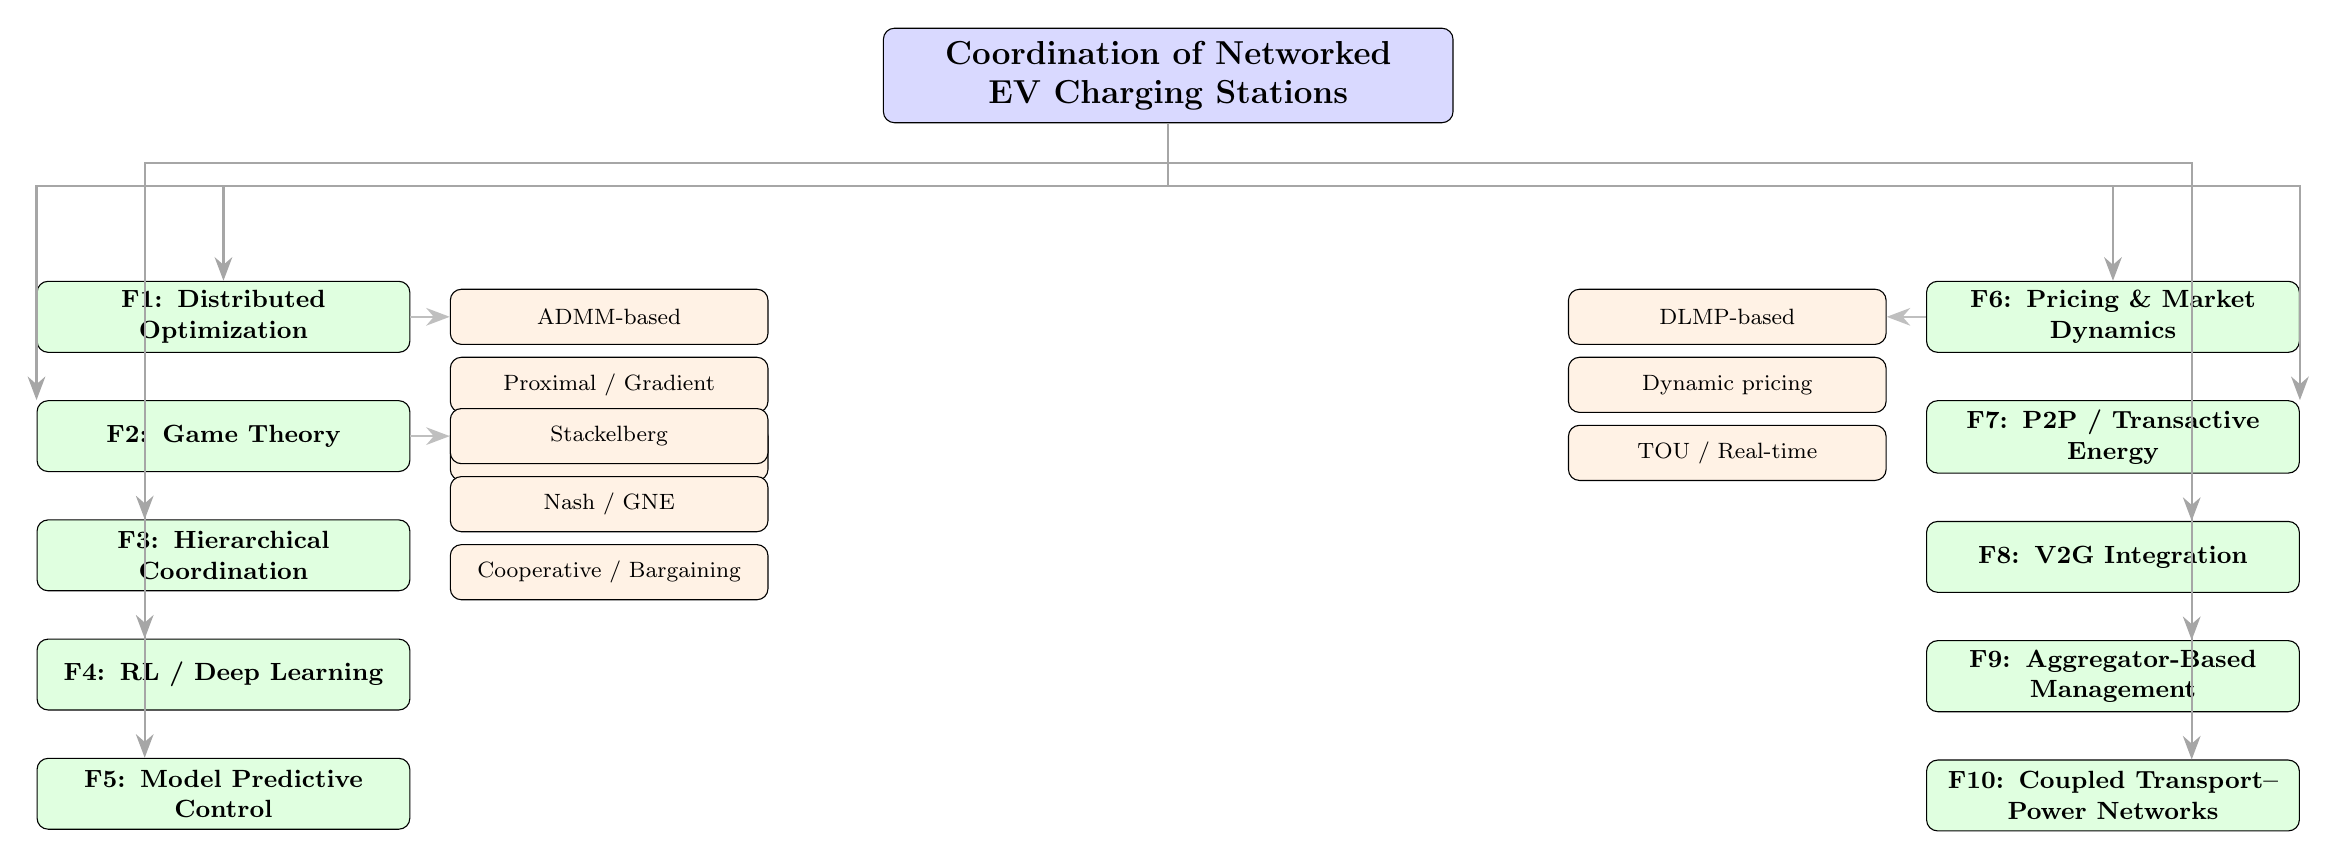
\begin{tikzpicture}[
    root/.style={rectangle, rounded corners, draw=black, fill=blue!15, text width=7cm, minimum height=1.2cm, text centered, font=\bfseries\large},
    level1/.style={rectangle, rounded corners, draw=black, fill=green!12, text width=4.5cm, minimum height=0.9cm, text centered, font=\small\bfseries},
    level2/.style={rectangle, rounded corners, draw=black, fill=orange!10, text width=3.8cm, minimum height=0.7cm, text centered, font=\footnotesize},
    arrow/.style={-{Stealth[length=3mm]}, thick, draw=gray!70}
]

% Root
\node[root] (root) {Coordination of Networked\\EV Charging Stations};

% Level 1 - Left column
\node[level1, below left=2.0cm and 6cm of root] (opt) {F1: Distributed\\Optimization};
\node[level1, below=0.6cm of opt] (game) {F2: Game Theory};
\node[level1, below=0.6cm of game] (hier) {F3: Hierarchical\\Coordination};
\node[level1, below=0.6cm of hier] (rl) {F4: RL / Deep Learning};
\node[level1, below=0.6cm of rl] (mpc) {F5: Model Predictive\\Control};

% Level 1 - Right column
\node[level1, below right=2.0cm and 6cm of root] (price) {F6: Pricing \& Market\\Dynamics};
\node[level1, below=0.6cm of price] (p2p) {F7: P2P / Transactive\\Energy};
\node[level1, below=0.6cm of p2p] (v2g) {F8: V2G Integration};
\node[level1, below=0.6cm of v2g] (agg) {F9: Aggregator-Based\\Management};
\node[level1, below=0.6cm of agg] (coupled) {F10: Coupled Transport--\\Power Networks};

% Level 2 - Sub-categories for key families
\node[level2, right=0.5cm of opt] (admm) {ADMM-based};
\node[level2, below=0.15cm of admm] (prox) {Proximal / Gradient};
\node[level2, below=0.15cm of prox] (sparse) {Sparsity-promoting};

\node[level2, right=0.5cm of game] (stack) {Stackelberg};
\node[level2, below=0.15cm of stack] (nash) {Nash / GNE};
\node[level2, below=0.15cm of nash] (coop) {Cooperative / Bargaining};

\node[level2, left=0.5cm of price] (dlmp) {DLMP-based};
\node[level2, below=0.15cm of dlmp] (dynp) {Dynamic pricing};
\node[level2, below=0.15cm of dynp] (tou) {TOU / Real-time};

% Arrows from root
\draw[arrow] (root.south) -- ++(0,-0.8) -| (opt.north);
\draw[arrow] (root.south) -- ++(0,-0.8) -| (game.north west);
\draw[arrow] (root.south) -- ++(0,-0.8) -| (price.north);
\draw[arrow] (root.south) -- ++(0,-0.8) -| (p2p.north east);

\draw[arrow] (root.south) -- ++(0,-0.5) -| ([xshift=-1cm]hier.north);
\draw[arrow] (root.south) -- ++(0,-0.5) -| ([xshift=-1cm]rl.north);
\draw[arrow] (root.south) -- ++(0,-0.5) -| ([xshift=-1cm]mpc.north);

\draw[arrow] (root.south) -- ++(0,-0.5) -| ([xshift=1cm]v2g.north);
\draw[arrow] (root.south) -- ++(0,-0.5) -| ([xshift=1cm]agg.north);
\draw[arrow] (root.south) -- ++(0,-0.5) -| ([xshift=1cm]coupled.north);

% Sub-arrows
\draw[arrow, gray!50] (opt.east) -- (admm.west);
\draw[arrow, gray!50] (game.east) -- (stack.west);
\draw[arrow, gray!50] (price.west) -- (dlmp.east);

\end{tikzpicture}
!!!!!}
\caption{Hierarchical taxonomy of methodological approaches for coordination of networked EV charging stations.}
\label{fig:taxonomy}
\end{figure}
\section{Research Gaps: What Exists Only in Simulation and Has Never Been Deployed on Real Cloud Infrastructure}

Despite the substantial body of literature on EV charging optimisation, 
a fundamental and largely overlooked divide exists between what has been 
proposed theoretically and what has actually been deployed on real 
cloud infrastructure. This section systematically identifies these gaps.

\subsection{ADMM-Based Distributed Coordination}

Distributed optimisation via ADMM has been extensively studied in 
simulation. Hierarchical frameworks combining the DSO, aggregators, 
and charging stations in multi-layer structures have been 
proposed~\cite{khaki2019hierarchical, zhang2022distributed, boyd2010admm}, 
and single-loop iterative algorithms have been developed to accelerate 
convergence~\cite{ma2013decentralized, yang2016distributed}. 
Nevertheless, all of these contributions are validated exclusively on 
local compute clusters or standard simulation benchmarks such as the 
IEEE 33-bus or 118-bus test systems. No published work deploys ADMM 
over a real cloud infrastructure---such as AWS or Azure---with actual 
network latency between geographically distributed stations and a 
remote coordination server. The fundamental question of how round-trip 
latency in the range of 50--200~ms affects ADMM convergence quality 
and real-time feasibility remains entirely unaddressed.

\subsection{Real-Time Optimisation with MPC}

Model Predictive Control has been applied to EV charging scheduling 
in both centralised and distributed 
variants~\cite{zheng2019online, gonzalez2021mpc, sen2024distributed}. 
However, these methods operate under the implicit assumption of 
zero-delay communication. As noted in the continuous-domain ADMM 
literature, iterative methods are highly sensitive to sampling time, 
and the impact of communication delays on real-time control 
performance has not been 
characterised~\cite{ma2016efficient, ardakanian2013distributed}. 
Deploying MPC over cloud infrastructure with realistic latency 
constraints remains an open problem.

\subsection{V2G Coordination at Scale}

Vehicle-to-Grid coordination using ADMM-based hierarchical frameworks 
has been proposed for large-scale 
settings~\cite{shao2021optimal, patil2021grid, shao2024decentralized}, 
with claims of scalability to high EV penetration levels. However, 
scalability in this context refers exclusively to simulation 
performance on benchmark networks. No work validates V2G coordination 
on real infrastructure with physical stations 
transmitting data to a cloud server under realistic communication 
conditions. The joint problem of V2G dispatch, battery degradation 
management~\cite{bashash2011plugin, wei2018ev}, and cloud-induced 
latency has never been addressed simultaneously.

\subsection{Federated Learning for EV Coordination}

Federated learning has recently emerged as a promising paradigm for 
privacy-preserving EV coordination. Edge-computing approaches for 
V2G dispatching have been 
explored~\cite{shang2022achieving, shang2024information}, and 
distributed deep reinforcement learning frameworks have been 
proposed~\cite{wan2019modelfree, li2020constrained, park2022multiagent}. 
However, existing federated approaches in the energy domain are 
primarily applied to supervised forecasting tasks, without addressing 
real-time reinforcement-based coordination under grid 
constraints~\cite{qiu2023rl}. Most multi-agent RL models for EVs 
assume synchronous agent behaviour and overlook privacy and fairness 
concerns in heterogeneous 
fleets~\cite{qian2022multiagent, wang2021rl}. Federated RL for 
real-time EV coordination, combining local policy training with 
global aggregation over a cloud server, remains at a very early stage 
and has never been validated on real deployment infrastructure.

\subsection{Privacy-Preserving Coordination}

Centralised coordination architectures require stations to share 
sensitive user data including location, driving patterns, and 
energy consumption profiles. Privacy-preserving variants of 
distributed coordination algorithms have been explored in a limited 
number of works~\cite{aravena2021decentralized, chowdhury2025secure}, 
but no deployed system currently addresses privacy leakage, 
cybersecurity risk, scalability, and regulatory compliance 
simultaneously at scale~\cite{sadeghian2022comprehensive, 
motlagh2025applied}. The trade-off between privacy budget and 
optimisation performance in the specific context of EV charging 
coordination is largely unexplored.

\subsection{What Cloud Platforms Currently Offer}

Existing industrial cloud deployments for EV charging---including 
AWS IoT Core-based architectures and ML-powered management 
platforms---are limited to operational management tasks such as 
remote monitoring, OCPP protocol handling, telemetry storage, 
transaction logging, and basic demand 
forecasting~\cite{shang2022achieving, sepehrzad2024applied}. 
No ADMM, MPC, or RL-based optimisation algorithm runs on these 
production cloud architectures. Edge computing has been explored 
for V2G dispatching using attention-based 
models~\cite{shang2022achieving}, but the integration of 
distributed optimisation algorithms within a real cloud 
orchestration stack, with latency-aware convergence guarantees, 
has not been demonstrated.

\subsection{Summary of Critical Gaps}

Table~\ref{tab:gaps} provides a structured overview of the gaps 
identified above.

\begin{table}[htbp]
\centering
\caption{Research gaps in cloud deployment of EV charging optimisation}
\label{tab:gaps}
\renewcommand{\arraystretch}{1.3}
\begin{tabular}{p{4.5cm} c c p{2.8cm}}
\toprule
\textbf{Research Area} & \textbf{Simulation} & \textbf{Cloud-Deployed} & \textbf{Gap Level} \\
\midrule
ADMM coordination~\cite{boyd2010admm, zhang2022distributed} 
    & \checkmark & $\times$ & Critical \\
ADMM + latency characterisation 
    & $\times$ & $\times$ & Critical \\
Asynchronous ADMM over cloud~\cite{aravena2021decentralized} 
    & Partial & $\times$ & Major \\
MPC real-time on cloud~\cite{zheng2019online, sen2024distributed} 
    & Partial & $\times$ & Major \\
V2G + ADMM at scale~\cite{shao2021optimal, patil2021grid} 
    & Partial & $\times$ & Major \\
Federated RL for coordination~\cite{shang2024information, park2022multiagent} 
    & Early & $\times$ & Major \\
Privacy-preserving coordination~\cite{aravena2021decentralized, chowdhury2025secure} 
    & $\times$ & $\times$ & Critical \\
ADMM + RL hybrid~\cite{pilco2023learning} 
    & $\times$ & $\times$ & Critical \\
Multi-energy coordination~\cite{guo2023hierarchical, long2022joint} 
    & Very rare & $\times$ & Major \\
Regulation-aware optimisation~\cite{motlagh2025applied} 
    & $\times$ & $\times$ & Major \\
Latency-aware cloud ADMM 
    & $\times$ & $\times$ & \textbf{PhD gap} \\
\bottomrule
\end{tabular}
\end{table}

These gaps collectively define the research space in which this 
thesis aims to make an original contribution, specifically targeting 
the design and experimental validation of a latency-aware, 
cloud-deployed distributed optimisation framework for large-scale 
EV charging coordination.

%% ============================================================
\section{Literature Review}\label{sec:review}
%% ============================================================

\subsection{Summary of Previously Published Reviews}\label{sec:prev_reviews}

\hspace{0.5cm}Table~\ref{tab:reviews} summarizes the coverage of previously published survey papers across six key dimensions: Model Predictive Control (MPC), Reinforcement Learning and real-time optimization (RL), Vehicle-to-Grid (V2G), Smart Charging, Pricing and Market Dynamics, and Cost Optimization. As shown, no single prior review comprehensively covers all six dimensions. The recent review by Ghanbari Motlagh et al.~\cite{motlagh2025applied} in \textit{Applied Energy} (2025) is the most comprehensive to date, yet it does not deeply address the scalability limitations of distributed optimization algorithms such as ADMM, nor does it explore bio-inspired or learning-augmented coordination paradigms.

\begin{table}[!htbp]
\centering
\caption{Summary of previously published reviews on EV charging coordination.}
\label{tab:reviews}
\footnotesize
\begin{tabular}{p{4cm}cccccc}
\toprule
\textbf{Reference(s)} & \textbf{MPC} & \textbf{RL} & \textbf{V2G} & \textbf{Smart} & \textbf{Pricing} & \textbf{Cost} \\
& & & & \textbf{Charging} & \textbf{\& Market} & \textbf{Optim.} \\
\midrule
Arias-Londo\~{n}o et al. (2020) & & & $\checkmark$ & $\checkmark$ & $\checkmark$ & \\
Sadeghian et al. (2022)~\cite{sadeghian2022comprehensive} & $\checkmark$ & & $\checkmark$ & $\checkmark$ & $\checkmark$ & $\checkmark$ \\
Chandra et al. (2024)~\cite{chandra2024comprehensive} & $\checkmark$ & & $\checkmark$ & $\checkmark$ & $\checkmark$ & $\checkmark$ \\
Qiu et al. (2023)~\cite{qiu2023rl} & & $\checkmark$ & $\checkmark$ & $\checkmark$ & & \\
Fescioglu-Unver et al. (2023)~\cite{fescioglu2023ev} & & $\checkmark$ & & $\checkmark$ & $\checkmark$ & \\
Pasha et al. (2024)~\cite{pasha2024ev} & & $\checkmark$ & $\checkmark$ & $\checkmark$ & $\checkmark$ & $\checkmark$ \\
Motlagh et al. (2025)~\cite{motlagh2025applied} & $\checkmark$ & $\checkmark$ & $\checkmark$ & $\checkmark$ & $\checkmark$ & $\checkmark$ \\
\midrule
\textbf{This report} & $\checkmark$ & $\checkmark$ & $\checkmark$ & $\checkmark$ & $\checkmark$ & $\checkmark$ \\
\bottomrule
\end{tabular}
\end{table}
\begin{tikzpicture}[scale=1.0]

% ===== CONFIGURATION =====
\def\maxrad{3.2}  % Reduced radius for smaller circles

% Angles: 6 axes, 60 degrees apart, starting from top (90) going clockwise
\def\angA{90}   % RL Real-Time Optimization
\def\angB{30}   % MPC
\def\angC{330}  % Cost Optimization
\def\angD{270}  % Pricing and Market Dynamics
\def\angE{210}  % Smart Charging
\def\angF{150}  % V2G

% Data values (out of 32 max)
\def\valA{9}    % RL Real-Time Optimization
\def\valB{8}    % MPC
\def\valC{26}   % Cost Optimization
\def\valD{22}   % Pricing and Market Dynamics
\def\valE{32}   % Smart Charging
\def\valF{22}   % V2G

% ===== GRID CIRCLES =====
\draw[gray!40, dashed, thin] (0,0) circle ({8/32*\maxrad});
\draw[gray!40, dashed, thin] (0,0) circle ({16/32*\maxrad});
\draw[gray!40, dashed, thin] (0,0) circle ({24/32*\maxrad});
\draw[black, thick] (0,0) circle (\maxrad);

% ===== AXES =====
\foreach \a in {\angA, \angB, \angC, \angD, \angE, \angF} {
    \draw[gray!60, thin] (0,0) -- (\a:\maxrad);
}

% ===== AXIS SCALE LABELS (along MPC axis at 30 degrees) =====
\node[below right, font=\small, inner sep=1pt] at (0.10, -0.04) {0};
\node[font=\small, inner sep=1pt] at (\angB:{8/32*\maxrad+0.15})  {8};
\node[font=\small, inner sep=1pt] at (\angB:{16/32*\maxrad+0.15}) {16};
\node[font=\small, inner sep=1pt] at (\angB:{24/32*\maxrad+0.15}) {24};
\node[font=\small, inner sep=1pt] at (\angB:{\maxrad+0.18})       {32};

% ===== AXIS LABELS =====
\node[above, font=\normalsize] 
    at (\angA:{\maxrad+0.25}) {RL Real-Time Optimization};
\node[right, font=\normalsize] 
    at (\angB:{\maxrad+0.35}) {MPC};
\node[below right, font=\normalsize, text width=3.0cm, align=center] 
    at (\angC:{\maxrad+0.3}) {Cost Optimization};
\node[below, font=\normalsize, text width=4.5cm, align=center] 
    at (\angD:{\maxrad+0.5}) {Pricing and Market Dynamics};
\node[left, font=\normalsize] 
    at (\angE:{\maxrad+0.4}) {Smart Charging};
\node[above left, font=\normalsize] 
    at (\angF:{\maxrad+0.35}) {V2G};

% ===== DATA POLYGON =====
\pgfmathsetmacro{\rA}{\valA/32*\maxrad}
\pgfmathsetmacro{\rB}{\valB/32*\maxrad}
\pgfmathsetmacro{\rC}{\valC/32*\maxrad}
\pgfmathsetmacro{\rD}{\valD/32*\maxrad}
\pgfmathsetmacro{\rE}{\valE/32*\maxrad}
\pgfmathsetmacro{\rF}{\valF/32*\maxrad}

\draw[blue!80!black, thick, fill=blue!10, fill opacity=0.4]
    (\angA:\rA) -- (\angB:\rB) -- (\angC:\rC) --
    (\angD:\rD) -- (\angE:\rE) -- (\angF:\rF) -- cycle;

% ===== DATA POINTS (filled circles) =====
\fill[blue!80!black] (\angA:\rA) circle (3pt);
\fill[blue!80!black] (\angB:\rB) circle (3pt);
\fill[blue!80!black] (\angC:\rC) circle (3pt);
\fill[blue!80!black] (\angD:\rD) circle (3pt);
\fill[blue!80!black] (\angE:\rE) circle (3pt);
\fill[blue!80!black] (\angF:\rF) circle (3pt);

% ===== LEGEND BOX =====
\node[draw=black, thin, fill=white, inner sep=6pt, font=\normalsize]
    at ({\maxrad+2.6}, 1.5) {
    \begin{tikzpicture}[baseline=-0.5ex]
        \draw[blue!80!black, thick] (0,0) -- (0.8,0);
        \fill[blue!80!black] (0,0) circle (2.5pt);
        \fill[blue!80!black] (0.8,0) circle (2.5pt);
        \node[right, font=\normalsize] at (-2.2,-1) {Number of papers};
    \end{tikzpicture}
};

% ===== FIGURE CAPTION =====
\node[font=\normalsize, text width=10cm, align=center]
    at (0,{-\maxrad-1.8}) {\textbf{Fig. 1.} Summary of previously published reviews.};

\end{tikzpicture}
%% ----------------------------------------------------------
\subsection{F1: Distributed Optimization}\label{sec:f1}
%% ----------------------------------------------------------

\hspace{0.5cm}Distributed optimization methods decompose the global charging coordination problem into local subproblems solved by individual stations or aggregators, linked through consensus constraints or shared coupling variables. The Alternating Direction Method of Multipliers (ADMM) has emerged as the dominant algorithmic framework~\cite{boyd2010admm}.

\hspace{0.5cm}Ma et al.~\cite{ma2013decentralized} proposed one of the earliest decentralized charging control schemes for large populations of plug-in EVs, using a valley-filling objective decomposed via dual methods. Subsequent work~\cite{ma2015distributed,ma2016efficient,ma2018charging} extended this framework to account for battery degradation costs, feeder capacity constraints, and improved computational efficiency. The ADMM framework was further applied by Khaki et al.~\cite{khaki2018hierarchical,khaki2019hierarchical} in a hierarchical setting combining exchange-based subproblem formulations.

\hspace{0.5cm}Zhang et al.~\cite{zhang2022distributed} introduced a distributed hierarchical coordination framework for networked charging stations incorporating peer-to-peer trading and EV charging flexibility quantification. While demonstrating strong theoretical performance, the authors acknowledged the computational burden of ADMM when the number of participating nodes increases significantly, motivating the scalability research addressed in this report.

\hspace{0.5cm}Other notable contributions include the sparsity-promoting distributed control of Li et al.~\cite{li2018sparsity}, the failure-tolerant optimization of Aravena et al.~\cite{aravena2021decentralized}, and the decentralized charging control with feeder overload management of Ghavami et al.~\cite{ghavami2016decentralized}. Chen et al.~\cite{chen2019extended} provided convergence guarantees for extended ADMM with nonseparable objectives, a formulation relevant to coupled charging station problems.


%% ----------------------------------------------------------
\subsection{F2: Game Theory}\label{sec:f2}
%% ----------------------------------------------------------

\hspace{0.5cm}Game-theoretic approaches model the strategic interactions among multiple self-interested agents---EVs, charging station operators, aggregators, and grid operators---each optimizing their own objectives subject to shared constraints.

\hspace{0.5cm}Wu et al.~\cite{wu2012v2a} formulated a vehicle-to-aggregator interaction game analyzing how EVs strategically choose charging and discharging actions. Gan et al.~\cite{gan2013optimal} designed an optimal decentralized protocol achieving a socially optimal charging profile as the Nash equilibrium of a non-cooperative game. Shakerighadi et al.~\cite{shakerighadi2018hierarchical} proposed a hierarchical game-theoretic approach combining Stackelberg and Nash equilibrium concepts across multiple levels.

\hspace{0.5cm}Stackelberg game formulations, where a leader (e.g., the grid operator or station owner) sets prices and followers (EVs) respond optimally, have been particularly popular~\cite{tan2017realtime,zhao2018realtime,guo2023hierarchical}. Cooperative game approaches, including Nash bargaining, have been used to ensure fair benefit allocation among networked stations~\cite{wang2020network,gao2024realtime}.

\hspace{0.5cm}Qian et al.~\cite{qian2022multiagent} introduced multi-agent deep reinforcement learning within a game-theoretic framework, bridging families F2 and F4. More recently, Qian et al.~\cite{qian2025trilevel} proposed a tri-level demand response framework for EVCS flexibility enhancement in coupled power and transportation networks.


%% ----------------------------------------------------------
\subsection{F3: Hierarchical Coordination}\label{sec:f3}
%% ----------------------------------------------------------

\hspace{0.5cm}Hierarchical coordination structures decompose the problem across multiple organizational or spatial levels---typically a grid-level coordinator, station-level schedulers, and individual EV controllers.

\hspace{0.5cm}Qi et al.~\cite{qi2014hierarchical} proposed hierarchical coordinated control for EV charging in multifamily dwellings. Xu et al.~\cite{xu2016hierarchical} developed a hierarchical framework specifically for China's charging infrastructure. Hu et al.~\cite{hu2016preventing} addressed distribution grid congestion through indirect control within a hierarchical management system. Sohet et al.~\cite{sohet2021hierarchical} presented a hierarchical coupled driving-and-charging model integrating EVs, stations, and grid operators.

\hspace{0.5cm}The hierarchical paradigm naturally combines with other families: hierarchical ADMM~\cite{khaki2018hierarchical}, hierarchical game theory~\cite{shakerighadi2018hierarchical,zhao2018realtime}, and hierarchical pricing~\cite{meng2024distributed}. Gonz\'alez-Garrido et al.~\cite{gonzalez2024hierarchical} recently proposed hierarchical control for collaborative EV charging to alleviate network congestion in constrained distribution networks.


%% ----------------------------------------------------------
\subsection{F4: Reinforcement Learning and Deep Learning}\label{sec:f4}
%% ----------------------------------------------------------

\hspace{0.5cm}Data-driven approaches, particularly reinforcement learning (RL) and deep reinforcement learning (DRL), have gained significant traction for real-time EV charging coordination due to their ability to handle uncertainty, non-stationarity, and high dimensionality without requiring explicit models.

\hspace{0.5cm}Wan et al.~\cite{wan2019modelfree} proposed model-free real-time scheduling based on DRL. Li et al.~\cite{li2020constrained} extended this with constrained DRL ensuring safe operation. Park and Moon~\cite{park2022multiagent} developed multi-agent DRL for charging scheduling in smart grids. Wang et al.~\cite{wang2021rl} applied RL to joint pricing and scheduling control. Zhang et al.~\cite{zhang2020effective} used DRL for effective charging planning considering driver behavior.

\hspace{0.5cm}Recent advances include hierarchical RL for navigation in coupled grids~\cite{jiang2024ev}, DRL for dynamic pricing of differentiated services~\cite{abdalrahman2022dynamic}, multi-objective RL for pricing~\cite{adetunji2024twotailed}, and multi-agent RL for flexible resource management~\cite{wu2024adaptive}. Critically for our research proposal, graph neural networks (GNNs) have been explored to learn structural properties of optimization problems, including accelerating ADMM convergence~\cite{pilco2023learning}.


%% ----------------------------------------------------------
\subsection{F5: Model Predictive Control}\label{sec:f5}
%% ----------------------------------------------------------

\hspace{0.5cm}Model Predictive Control (MPC) provides a rolling-horizon optimization framework that naturally handles dynamic constraints, forecasting uncertainties, and multi-step decision-making. Zheng et al.~\cite{zheng2019online} proposed online distributed MPC for optimal scheduling of EV charging stations. Gonzalez-Rivera et al.~\cite{gonzalez2021mpc} applied MPC to hybrid charging stations. Sen and Kumar~\cite{sen2024distributed} developed distributed-MPC for renewables and EVs in building-integrated microgrids. While MPC offers principled handling of dynamics and constraints, its computational cost scales with the prediction horizon and problem dimension, making real-time implementation challenging for large networks.


%% ----------------------------------------------------------
\subsection{F6: Pricing and Market Dynamics}\label{sec:f6}
%% ----------------------------------------------------------

\hspace{0.5cm}Pricing mechanisms serve as implicit coordination signals that align the interests of self-interested agents with system-level objectives. Distribution Locational Marginal Prices (DLMPs) capture the marginal cost of energy at each node, providing spatially differentiated price signals~\cite{wang2023dlmp,patnam2021dlmp}.

\hspace{0.5cm}Dynamic pricing strategies have been developed for various objectives: congestion management~\cite{kazemtarghi2024dynamic}, revenue maximization~\cite{ye2023identifying}, cooperative alliances~\cite{gao2024realtime}, and hierarchical pricing mechanisms~\cite{meng2024distributed}. Liu et al.~\cite{liu2019twostage} proposed two-stage transactive control scheduling. Affolabi et al.~\cite{affolabi2022optimal} optimized transactive energy trading with on-site PV generation.

\hspace{0.5cm}Table~\ref{tab:game_pricing} summarizes the recent game-based pricing approaches in the literature, adapted and extended from the comprehensive review of Ghanbari Motlagh et al.~\cite{motlagh2025applied}.


\begin{table}[!htbp]
\centering
\caption{Summary of recent papers on game-based pricing for EV charging coordination.}
\label{tab:game_pricing}
\footnotesize
\begin{tabular}{p{1.5cm}cp{2.5cm}p{4.5cm}p{3.5cm}}
\toprule
\textbf{Ref.} & \textbf{Year} & \textbf{Game Type} & \textbf{Main Objective} & \textbf{Players} \\
\midrule
\cite{affolabi2022optimal} & 2022 & Cooperative (Nash Bargaining) & Maximize payoff of EVCSs and EVs; fair benefit allocation & EVCSs, individual EVs \\
\addlinespace
\cite{guo2023hierarchical} & 2023 & Stackelberg & Optimize hydrogen trading prices; maximize revenue & Hydrogen provider (leader), HFSs (followers) \\
\addlinespace
\cite{wang2020network} & 2020 & GNE & Maximize utility of active load aggregators under network constraints & EV aggregators competing for energy \\
\addlinespace
\cite{najafi2022optimal} & 2022 & Bilevel & Upper: maximize DG hosting; Lower: maximize EV aggregator profit & DISCO, EV aggregator, EV owners \\
\addlinespace
\cite{kazemtarghi2024dynamic} & 2024 & Stackelberg & Achieve win--win for retailers and EV users via hybrid demand response & Retailers (leader), EV users (followers) \\
\addlinespace
\cite{gao2024realtime} & 2024 & Cooperative & Real-time pricing strategy for fast charging station alliance based on DLMP & Fast charging stations alliance, EV users \\
\addlinespace
\cite{qian2025trilevel} & 2025 & Stackelberg & Tri-level demand response for EVCS flexibility in coupled networks & EVCSs, DSO, transmission operator \\
\bottomrule
\end{tabular}
\end{table}



%% ----------------------------------------------------------
\subsection{F7: Peer-to-Peer and Transactive Energy}\label{sec:f7}
%% ----------------------------------------------------------

\hspace{0.5cm}Peer-to-peer (P2P) energy trading enables direct energy exchange between charging stations, microgrids, or prosumers without centralized intermediation. Zhang et al.~\cite{zhang2022distributed} integrated P2P trading within the distributed hierarchical coordination of networked stations. Yan and Chen~\cite{yan2023distributed,yan2023coordination} proposed distributed online algorithms for promoting energy sharing between stations, including configurations with shared energy storage.

\hspace{0.5cm}Blockchain-based approaches have been explored for securing P2P transactions~\cite{ping2021twostage,chowdhury2025secure}. Vehicle-to-vehicle (V2V) energy swapping has also been studied~\cite{wang2018spatio,zeng2021hierarchical}. Zhong et al.~\cite{zhong2019topology} developed topology-aware V2G trading for active distribution systems.


%% ----------------------------------------------------------
\subsection{F8: Vehicle-to-Grid Integration}\label{sec:f8}
%% ----------------------------------------------------------

\hspace{0.5cm}Vehicle-to-Grid (V2G) technology enables bidirectional power flow between EVs and the grid, allowing EVs to provide ancillary services such as frequency regulation, voltage support, and peak shaving~\cite{patil2021grid}. Shao et al.~\cite{shao2021optimal} addressed optimal stochastic operation integrating V2G with renewable energy and hydrogen systems. Edge computing architectures have been proposed for efficient V2G dispatching~\cite{shang2022achieving,shang2024information}.


%% ----------------------------------------------------------
\subsection{F9: Aggregator-Based Management}\label{sec:f9}
%% ----------------------------------------------------------

\hspace{0.5cm}Aggregators serve as intermediaries that pool the flexibility of multiple EVs to participate in wholesale or distribution-level markets. Gupta et al.~\cite{gupta2019collaborative} addressed collaborative multi-aggregator scheduling. Ding et al.~\cite{ding2020spatial} developed spatial-temporal demand management for geo-distributed stations and aggregators. Wei et al.~\cite{wei2020aggregation} modeled aggregation considering power fluctuations and load rebound. Alsabbagh et al.~\cite{alsabbagh2021distributed} incorporated time anxiety and customer behaviors.

\hspace{0.5cm}Pan et al.~\cite{pan2020stochastic} proposed stochastic transactive control for EV aggregator coordination using decentralized approximate dynamic programming. Mohiti et al.~\cite{mohiti2019distributed} developed a distributed robust model for the coordinated operation of smart distribution networks and EV aggregators.


%% ----------------------------------------------------------
\subsection{F10: Coupled Transportation--Power Networks}\label{sec:f10}
%% ----------------------------------------------------------

\hspace{0.5cm}This family considers the joint optimization of transportation routing and power grid operations, recognizing that EV charging decisions affect both traffic flow and power distribution. Sun et al.~\cite{sun2019ev} addressed EV scheduling in coupled transportation--power networks. Guo et al.~\cite{guo2014rapid} proposed real-time rapid-charging navigation using both power system and traffic data. Qian et al.~\cite{qian2020enhanced} enhanced coordinated operations of electric power and transportation networks. More recently, Shao et al.~\cite{shao2024decentralized} proposed a decentralized bi-level decomposition for optimal operation in coupled urban systems, and Qian et al.~\cite{qian2025unsupervised} applied unsupervised learning for efficient load and traffic flow distribution.



%% ============================================================
\section{Comparative Analysis}\label{sec:comparison}
%% ============================================================

\hspace{0.5cm}Table~\ref{tab:comparison} provides a comprehensive comparison of the ten methodological families across key evaluation criteria: optimization architecture, communication requirements, scalability, real-time capability, consideration of uncertainty, and ability to handle network constraints.

\begin{table}[!htbp]
\centering
\caption{Comparative analysis of methodological families for networked EV charging coordination.}
\label{tab:comparison}
\footnotesize
\begin{tabular}{p{1.8cm}p{1.5cm}p{1.5cm}p{1.3cm}p{1.3cm}p{1.5cm}p{1.5cm}p{1.8cm}}
\toprule
\textbf{Family} & \textbf{Architecture} & \textbf{Comm.} & \textbf{Scala- bility} & \textbf{Real- time} & \textbf{Uncer- tainty} & \textbf{Network constr.} & \textbf{Key limitation} \\
\midrule
F1: Distrib. Optim. & Decentral. & Iterative & Low--Med & Low & Limited & Yes & Slow convergence at scale \\
\addlinespace
F2: Game Theory & Mixed & Varies & Medium & Medium & Partial & Partial & Equilibrium existence \\
\addlinespace
F3: Hierarchical & Multi-level & Top-down & Medium & Medium & Partial & Yes & Communication bottleneck \\
\addlinespace
F4: RL / DL & Decentral. & Minimal & High & High & Yes & Implicit & Training cost; safety \\
\addlinespace
F5: MPC & Central. & Periodic & Low & Medium & Yes & Yes & Computational cost \\
\addlinespace
F6: Pricing & Decentral. & Price signal & High & High & Partial & DLMP & Price volatility \\
\addlinespace
F7: P2P / Trans. & Peer-based & Bilateral & Medium & Medium & Limited & Partial & Trust; settlement \\
\addlinespace
F8: V2G & Mixed & Bidirect. & Medium & High & Partial & Yes & Battery degradation \\
\addlinespace
F9: Aggregator & Central./agg. & Aggregated & Medium & Medium & Partial & Indirect & Aggregator dependency \\
\addlinespace
F10: Coupled & Central. & Extensive & Low & Low & Limited & Yes & Extreme complexity \\
\bottomrule
\end{tabular}
\end{table}
\section{Vehicle-to-Grid (V2G) and Frequency Regulation}

\subsection{Grid Frequency: Fundamentals}

The European electrical grid operates at a nominal frequency of 50~Hz. 
This frequency reflects the real-time balance between generation and consumption:

\begin{itemize}
    \item Generation = Consumption $\Rightarrow$ frequency = 50~Hz
    \item Generation $>$ Consumption $\Rightarrow$ frequency rises above 50~Hz
    \item Generation $<$ Consumption $\Rightarrow$ frequency drops below 50~Hz
\end{itemize}

Significant deviations from this nominal value can have severe consequences 
for grid stability. A frequency drop to 49.5~Hz triggers automatic alarms, 
while a sustained drop to 48.5~Hz can lead to widespread blackouts.

\subsection{Motivation: The Challenge of Renewable Integration}

Traditionally, frequency regulation was naturally provided by large thermal 
power plants, whose rotating masses offer significant mechanical inertia that 
absorbs frequency disturbances automatically. However, the increasing 
penetration of renewable energy sources such as solar photovoltaic and wind 
power introduces a fundamental challenge: these sources provide little to no 
rotational inertia, making the grid increasingly vulnerable to frequency 
deviations. As the share of renewables grows, alternative sources of fast 
frequency response become critical.

\subsection{EVs as Frequency Regulation Assets}

Each grid-connected EV equipped with bidirectional charging capability 
constitutes a fast-responding distributed energy resource. Unlike thermal 
generators, which require 30 seconds to several minutes to adjust their output, 
EV batteries can respond to frequency signals within 100--500~ms, making them 
particularly well-suited for primary frequency regulation.

The response mechanism is straightforward. Let $\Delta f = f_{\text{measured}} 
- 50$~Hz denote the frequency deviation. Each station $i$ computes a 
regulation power signal proportional to this deviation:

\begin{equation}
    p_i^{\text{reg}} = -K_i \cdot \Delta f
\end{equation}

where $K_i$ is the droop coefficient of station $i$, expressing its 
sensitivity to frequency deviations. A negative deviation (under-frequency) 
triggers power injection into the grid (discharging), while a positive 
deviation (over-frequency) triggers increased absorption (charging).

Before responding, each station verifies local feasibility constraints:

\begin{itemize}
    \item Current SoC exceeds the minimum admissible threshold
    \item Requested power does not exceed the hardware rating $p_i^{\max}$
    \item Remaining time before EV departure is sufficient to allow discharging
\end{itemize}

\subsection{Ancillary Service Categories}

Grid-connected EVs can participate in three categories of frequency 
regulation services, each with distinct response time requirements 
and remuneration levels:

\begin{itemize}
    \item \textbf{Primary Frequency Regulation (PFR):} Automatic, 
    near-instantaneous response to frequency deviations, required within 
    30~seconds. This is the most critical and best-remunerated service.

    \item \textbf{Secondary Frequency Regulation (SFR):} Restores frequency 
    precisely to 50~Hz following primary response, with activation times 
    between 30~seconds and 15~minutes, controlled by the transmission 
    system operator.

    \item \textbf{Tertiary Regulation:} A pre-scheduled reserve activated 
    over horizons exceeding 15~minutes, less critical and carrying lower 
    remuneration.
\end{itemize}

\subsection{Benefits of V2G Frequency Regulation}

V2G participation in frequency regulation delivers benefits across 
multiple stakeholders:

\begin{itemize}
    \item \textbf{For the grid operator:} Enhanced stability under high 
    renewable penetration, reduced reliance on polluting and costly 
    thermal spinning reserves, and access to a geographically distributed 
    fast-response resource with no single point of failure.

    \item \textbf{For EV owners:} Estimated ancillary service revenues 
    of 100--300~\euro/year, with the vehicle generating income during 
    idle parking periods without requiring manual intervention.

    \item \textbf{For charging station operators:} Access to ancillary 
    service markets and improved asset utilisation through monetisation 
    of fleet flexibility.
\end{itemize}

\subsection{The Central Trade-off: Revenue vs. Battery Degradation}

The fundamental challenge of V2G frequency regulation lies in the 
accelerated battery degradation induced by frequent charge-discharge 
cycling. Each station $i$ must therefore solve a local optimisation 
problem that explicitly accounts for this trade-off:

\begin{equation}
    \max_{p_i} \quad R_i(p_i) - D_i(p_i) - U_i(p_i)
\end{equation}

where $R_i(p_i)$ denotes the regulation revenue, $D_i(p_i)$ the battery 
degradation cost, and $U_i(p_i)$ a penalty for user dissatisfaction 
arising from SoC depletion prior to departure. Given that EV battery 
replacement costs range from 5,000 to 15,000~\euro, the net benefit of 
V2G participation is not always guaranteed, and its quantification 
requires accurate degradation models.

\subsection{Role of ADMM in V2G Coordination}

Without coordination, individual stations acting independently may 
over-discharge, fail to meet the aggregate regulation target, or 
create voltage imbalances in the distribution network. ADMM provides 
a principled framework for distributed V2G coordination: upon receiving 
the frequency deviation signal $\Delta f$, the cloud coordinator 
broadcasts a dual variable $\lambda$ to all stations, each of which 
then solves its local subproblem accounting for SoC constraints, 
departure time, and degradation cost. Iterative exchange of local 
power decisions and global signals drives the fleet toward a 
collectively feasible and optimal regulation response.



%% ============================================================
\section{Research Gaps}\label{sec:gaps}
%% ============================================================

\hspace{0.5cm}Based on the comprehensive review, we identify the following critical research gaps:

\hspace{0.5cm}\textbf{Gap~1: Scalability of ADMM-based Distributed Coordination.}
The ADMM algorithm, while providing convergence guarantees for convex problems and enabling privacy-preserving distributed computation, suffers from a fundamental scalability limitation. As documented in~\cite{zhang2022distributed}, when the number of networked stations grows beyond a few dozen, the number of ADMM iterations required for convergence increases substantially, and each iteration involves communication rounds between all participating agents. The penalty parameter $\rho$, step sizes, and other algorithmic hyperparameters are typically fixed or manually tuned, which is suboptimal for heterogeneous and time-varying network conditions. No existing work in the EV charging domain has addressed this through learning-based parameter adaptation.

\begin{comment}
\textbf{\hspace{0.5cm}\textbf{Gap~2: Absence of Bio-Inspired Decentralized Coordination.}
Despite the inherently distributed and self-organizing nature of the charging station coordination problem, no existing work has explored bio-inspired coordination mechanisms---such as reaction--diffusion systems, swarm intelligence, or stigmergic coordination---for EV charging. These mechanisms are well-studied in biological systems for achieving emergent global coordination through purely local interactions, which is precisely the paradigm needed for scalable real-time coordination. 
}  
\end{comment}



\hspace{0.5cm}\textbf{Gap~2: Integration Gap Between Theory and Cloud Deployment.}
Most distributed optimization methods are validated through numerical simulations on standard test networks. There is a significant gap between these theoretical demonstrations and real-world deployment on cloud/edge infrastructure with realistic communication latencies, data asynchrony, and fault tolerance requirements.

\hspace{0.5cm}\textbf{Gap~3: Lack of Cross-Family Integration.}
While individual methodological families have matured significantly, there is limited work on systematically combining their strengths---for example, using RL to learn optimal parameters for distributed optimization algorithms.

\hspace{0.5cm}\textbf{Gap~4: Real-Time Flexibility Quantification at Network Scale.}
The quantification of aggregate charging flexibility across an entire network of stations in real time, accounting for individual EV constraints, battery degradation, and driver preferences, remains an open challenge~\cite{massaoudi2025analysis,harighi2024flexibility}.


%% ============================================================
\section{Research Proposals}\label{sec:proposal}
%% ============================================================



%% ----------------------------------------------------------
\subsection{Piste~1: RL/GNN-Accelerated ADMM for Large-Scale Coordination}\label{sec:piste1}
%% ----------------------------------------------------------

\subsubsection{Motivation}

\hspace{0.5cm}The standard ADMM algorithm for coordinating $N$ networked charging stations solves at each iteration $k$:
\begin{align}
    x_i^{k+1} &= \arg\min_{x_i} \left\{ f_i(x_i) + \frac{\rho}{2}\left\| x_i - z^k + u_i^k \right\|_2^2 \right\}, \quad \forall\, i = 1,\ldots,N, \label{eq:admm_x} \\
    z^{k+1} &= \arg\min_z \left\{ g(z) + \frac{N\rho}{2}\left\| z - \bar{x}^{k+1} - \bar{u}^k \right\|_2^2 \right\}, \label{eq:admm_z} \\
    u_i^{k+1} &= u_i^k + x_i^{k+1} - z^{k+1}, \quad \forall\, i = 1,\ldots,N, \label{eq:admm_u}
\end{align}
where $f_i(\cdot)$ represents the local cost function of station $i$, $g(\cdot)$ encodes the coupling constraints (grid capacity, power flow), $\rho$ is the penalty parameter, and $u_i$ are scaled dual variables. The convergence rate critically depends on $\rho$ and is known to degrade as $N$ increases.

\subsubsection{Proposed Approach}

\hspace{0.5cm}We propose to learn a mapping $\pi_\theta: \mathcal{G}^k \rightarrow (\rho^{k+1}, \alpha^{k+1})$ that, given the current state of the optimization encoded as a graph $\mathcal{G}^k = (\mathcal{V}, \mathcal{E}, \mathbf{H}^k)$, predicts optimal ADMM parameters for the next iteration. Here:
\begin{itemize}
    \item $\mathcal{V} = \{1,\ldots,N\}$ represents charging stations as nodes;
    \item $\mathcal{E}$ captures the electrical and communication topology;
    \item $\mathbf{H}^k = [h_1^k, \ldots, h_N^k]$ are node features encoding primal residuals, dual residuals, local costs, and constraint violations at iteration $k$.
\end{itemize}

\hspace{0.5cm}The GNN architecture uses message-passing layers:
\begin{equation}
    h_i^{(l+1)} = \phi\left( h_i^{(l)}, \bigoplus_{j \in \mathcal{N}(i)} \psi\left(h_i^{(l)}, h_j^{(l)}, e_{ij}\right) \right),
    \label{eq:gnn}
\end{equation}
where $\phi$ and $\psi$ are learnable functions, $\bigoplus$ is a permutation-invariant aggregation, and $e_{ij}$ are edge features (line impedances, capacity limits). The RL agent is trained with a reward signal:
\begin{equation}
    r^k = -\left( \left\| r_{\text{primal}}^k \right\|_2 + \left\| r_{\text{dual}}^k \right\|_2 \right) - \lambda \cdot k,
    \label{eq:reward}
\end{equation}
where the first term rewards convergence progress and the second term penalizes iteration count.

\subsubsection{Expected Contributions}

\hspace{0.5cm}This approach is expected to: (i)~reduce the number of ADMM iterations by 50--80\% for networks with $N > 50$ stations; (ii)~maintain convergence guarantees through a safeguard mechanism that reverts to standard ADMM if the learned parameters violate sufficient descent conditions; and (iii)~generalize across different network topologies through the GNN's inductive bias.


%% ----------------------------------------------------------
\subsection{Piste~2: Bio-Inspired Reaction--Diffusion Coordination Framework}\label{sec:piste2}
%% ----------------------------------------------------------

\subsubsection{Motivation and Bio-Inspired Analogy}

\hspace{0.5cm}In biological systems, Turing-type reaction--diffusion (RD) mechanisms produce stable spatial patterns through the interaction of a short-range activator and a long-range inhibitor~\cite{turing1952chemical,kondo2010reaction}. We propose an original analogy: \textit{charging stations are biological cells that self-organize through local price--charge signaling}, where:
\begin{itemize}
    \item \textbf{Activator ($a_i$):} The local electricity price at station $i$, which tends to attract EVs (high price at neighbors pushes demand to station $i$);
    \item \textbf{Inhibitor ($b_i$):} The local charging load or congestion level, which diffuses over the network and suppresses demand at overloaded stations.
\end{itemize}

\hspace{0.5cm}The key insight is that the interplay between these two signals---one promoting and one suppressing local charging demand---can produce emergent, stable, and globally efficient allocation patterns without any central coordinator, analogous to how Turing patterns emerge in embryonic development.

\subsubsection{Mathematical Formulation}

\hspace{0.5cm}The dynamics at each station $i \in \{1,\ldots,N\}$ are governed by a coupled reaction--diffusion system:
\begin{align}
    \frac{\partial a_i}{\partial t} &= D_a \sum_{j \in \mathcal{N}(i)} w_{ij}(a_j - a_i) + f(a_i, b_i; \theta_f), \label{eq:rd_a} \\
    \frac{\partial b_i}{\partial t} &= D_b \sum_{j \in \mathcal{N}(i)} w_{ij}(b_j - b_i) + g(a_i, b_i; \theta_g), \label{eq:rd_b}
\end{align}
where:
\begin{itemize}
    \item $D_a, D_b > 0$ are diffusion coefficients with $D_b \gg D_a$ (the inhibitor diffuses faster, a necessary condition for Turing instability);
    \item $w_{ij}$ are edge weights reflecting the electrical/geographic proximity between stations $i$ and $j$;
    \item $f(\cdot; \theta_f)$ and $g(\cdot; \theta_g)$ are the local reaction kinetics, parameterized by learnable vectors $\theta_f$ and $\theta_g$.
\end{itemize}

\hspace{0.5cm}The reaction functions encode the local market dynamics:
\begin{align}
    f(a_i, b_i; \theta_f) &= \theta_{f,1}\, a_i(1 - a_i) - \theta_{f,2}\, a_i\, b_i + \theta_{f,3}\,(d_i - s_i), \label{eq:f_reaction} \\
    g(a_i, b_i; \theta_g) &= \theta_{g,1}\, a_i^2 - \theta_{g,2}\, b_i + \theta_{g,3}\, c_i^{\text{grid}}, \label{eq:g_reaction}
\end{align}
where $d_i$ is the local EV demand, $s_i$ is the available supply (including on-site PV/storage), and $c_i^{\text{grid}}$ represents grid-side constraints (feeder capacity, voltage bounds).

\subsubsection{Differentiable Parameter Optimization Pipeline}

\hspace{0.5cm}The RD parameters $\Theta = (D_a, D_b, \theta_f, \theta_g)$ are learned from historical operational data through a differentiable optimization pipeline. The RD dynamics~\eqref{eq:rd_a}--\eqref{eq:rd_b} are discretized using an explicit Euler scheme:
\begin{align}
    a_i^{t+1} &= a_i^t + \Delta t \left[ D_a \sum_{j} w_{ij}(a_j^t - a_i^t) + f(a_i^t, b_i^t; \theta_f) \right], \\
    b_i^{t+1} &= b_i^t + \Delta t \left[ D_b \sum_{j} w_{ij}(b_j^t - b_i^t) + g(a_i^t, b_i^t; \theta_g) \right].
\end{align}

\hspace{0.5cm}Since the entire forward pass is differentiable with respect to $\Theta$, we define a loss function that penalizes deviations from historical optimal allocations and grid constraint violations:
\begin{equation}
    \mathcal{L}(\Theta) = \sum_{t=1}^{T} \left[ \alpha \left\| \mathbf{a}^t(\Theta) - \mathbf{a}^{t,*} \right\|_2^2 + \beta \sum_{i} \max\left(0, b_i^t(\Theta) - \bar{b}_i\right)^2 \right],
    \label{eq:loss}
\end{equation}
where $\mathbf{a}^{t,*}$ are the historical optimal price allocations and $\bar{b}_i$ is the capacity limit at station $i$. The parameters are updated via gradient descent:
\begin{equation}
    \Theta \leftarrow \Theta - \eta \nabla_\Theta \mathcal{L}(\Theta),
    \label{eq:gradient}
\end{equation}
with gradients computed through automatic differentiation (backpropagation through the discretized dynamics).

\subsubsection{Cloud Infrastructure Architecture}

\hspace{0.5cm}The framework is designed for deployment on a production AWS cloud infrastructure:

\begin{itemize}
    \item \textbf{AWS IoT Core:} MQTT-based real-time communication between physical charging stations and the cloud, enabling low-latency collection of $(a_i, b_i, d_i, s_i)$ signals.
    \item \textbf{AWS Lambda:} Serverless compute functions executing the local RD update equations~\eqref{eq:rd_a}--\eqref{eq:rd_b} for each station in parallel, triggered by incoming IoT messages.
    \item \textbf{AWS DynamoDB:} NoSQL database storing station states, parameters $\Theta$, historical trajectories, and neighbor information $w_{ij}$.
    \item \textbf{AWS Step Functions:} Orchestration of the differentiable optimization pipeline---periodic batch learning of $\Theta$ from accumulated operational data, with automatic rollback if performance degrades.
\end{itemize}

\hspace{0.5cm}This architecture supports horizontal scaling: adding a new station requires only deploying a new IoT endpoint and Lambda function, without modifying the coordination logic. The purely local nature of the RD computations ensures that latency does not grow with network size.

\subsubsection{Advantages Over ADMM}

\begin{table}[!htbp]
\centering
\caption{Comparison between ADMM-based coordination and the proposed RD framework.}
\label{tab:admm_vs_rd}
\footnotesize
\begin{tabular}{p{3.5cm}p{4.5cm}p{4.5cm}}
\toprule
\textbf{Criterion} & \textbf{Standard ADMM} & \textbf{Proposed RD Framework} \\
\midrule
Communication & Iterative all-to-coordinator & Local neighbor-only \\
Convergence & Guaranteed (convex) & Emergent (learned stability) \\
Scalability & $O(N \cdot K)$ per round & $O(|\mathcal{N}|)$ per station \\
Real-time capability & Limited (many iterations) & High (continuous dynamics) \\
Parameter tuning & Manual / fixed $\rho$ & Learned via differentiable optim. \\
Fault tolerance & Coordinator failure = system failure & Graceful degradation \\
Cloud deployment & Complex orchestration & Native serverless fit \\
\bottomrule
\end{tabular}
\end{table}



%% ============================================================
\section{Conclusion}\label{sec:conclusion}
%% ============================================================

\hspace{0.5cm}This report has presented a comprehensive literature review of the coordination of networked EV charging stations, classifying over 100 references into ten methodological families and providing detailed comparative analysis through structured tables and a taxonomy diagram. The critical analysis of the literature has revealed several important research gaps, most notably the scalability limitations of ADMM-based distributed optimization and the absence of bio-inspired coordination paradigms in this domain.

\hspace{0.5cm}To address these gaps, we have proposed two complementary research directions. The first direction leverages graph neural networks and reinforcement learning to adaptively tune ADMM parameters, accelerating convergence for large-scale networks while preserving theoretical guarantees. The second direction introduces an original bio-inspired framework based on Turing-type reaction--diffusion dynamics, where charging stations self-organize as cells through local activator--inhibitor (price--charge) interactions, with parameters learned through a differentiable optimization pipeline and the entire system deployed on AWS cloud infrastructure.

\hspace{0.5cm}These two directions are complementary: Piste~1 improves existing methods incrementally, providing a near-term solution, while Piste~2 proposes a paradigm shift toward emergent, cloud-native coordination that may define the next generation of large-scale EV charging management systems.


%% ============================================================
% Bibliography
%% ============================================================
\bibliographystyle{elsarticle-num}
\bibliography{references}

\end{document}